14. \begin{figure}[ht!]
\center{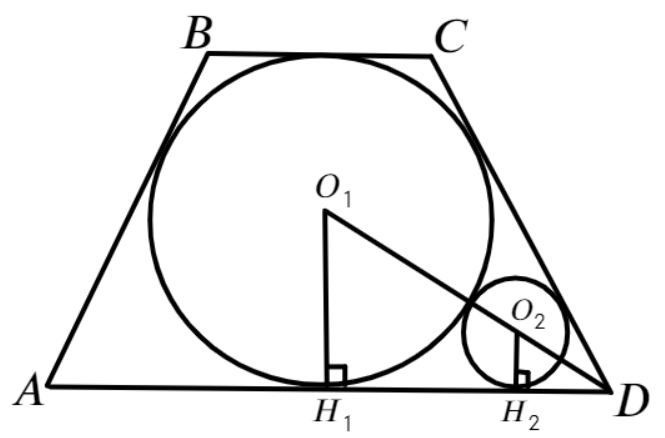
\includegraphics[scale=0.35]{g9-13.png}}
\end{figure}\\
Высота трапеции в два раза больше радиуса вписанной окружности и равна $2\cdot4=8.$ Пусть меньшее основания равны $a$ и $b,\ a>b,$ тогда опустив две высоты из точек $B$ и $C,$ найдём $\cfrac{a-b}{2}=\sqrt{100-64}=6,\ a-b=12.$ Так как трапеция является описанной, $a+b=10+10=20,$ откуда $2a=12+20=32,\ a=16,\ b=16-12=4.$ Раз обе окружности касаются сторон $AD$ и $CD,$ их центры лежат на биссектрисе угла $D.$ Проведём перпендикуляры $O_1H_1$ и $O_2H_2$ к точкам касания. Найдём $O_1D=\sqrt{8^2+4^2}=4\sqrt{5}.$ Пусть радиус меньшей окружности равен $x,$ тогда  $O_2D=4\sqrt{5}-4-x.$ Из подобия треугольников $O_1H_1D$ и $O_2H_2D$ (по двум углам) получаем соотношение $\cfrac{4\sqrt{5}-4-x }{4\sqrt{5}}=\cfrac{x}{4},$ откуда $16\sqrt{5}-16-4x=4\sqrt{5}x,\ 4x(1+\sqrt{5})=16(\sqrt{5}-1),\ x=\cfrac{4(\sqrt{5}-1)}{1+\sqrt{5}}=6-2\sqrt{5}.$\\
